\resourceheading{8}{Low-Tech AAC Backup \& Vocabulary Starter}{AAC continuity and multimodal communication\par}{Communicators, families, teachers, speech-language pathologists \& support staff}{Module 3 multimodal system, AAC review, and EDU486 sensory feedback}

\vspace{-0.5cm}
\toolsection{What This Resource Is}

A shared record can preserve meaning only if the communicator can still express it when the primary route is unavailable. A low-tech backup is a printed or durable communication display that preserves access when a speech-generating device is charging, unavailable, difficult to position, unsafe near materials, or simply not preferred in that moment. It is not a lesser system or a test a learner must pass before ``earning'' technology. Multimodal AAC combines aided and unaided methods, and the available route should change with the communicator's needs, preferences, and context without reducing the range of messages they can express \citep{ashaAAC,mirenda2015aids}. The starter below organizes vocabulary by communicative function rather than by adult task. The communicator and speech-language pathologist should determine representation, language, field size, layout, symbol system, color, spacing, contrast, and access method. When useful for motor planning, important vocabulary should remain in predictable locations across the primary and backup systems.

\toolsection{Core, Context, and Repair Starter}

\renewcommand{\arraystretch}{1.00}
\setlength{\tabcolsep}{3pt}

\begin{tabularx}{\textwidth}{|>{\centering\arraybackslash}p{0.60in}|>{\centering\arraybackslash}p{0.70in}|>{\centering\arraybackslash}p{0.70in}|>{\centering\arraybackslash}X|>{\centering\arraybackslash}X|>{\centering\arraybackslash}X|}
\hline
\rowcolor{SoftBlue}
\textbf{I} & \textbf{you} & \textbf{it} & \textbf{want} & \textbf{not} & \textbf{more} \\
\hline

\rowcolor{SoftGreen}
\textbf{go} & \textbf{stop} & \textbf{help} & \textbf{look} & \textbf{think} & \textbf{like} \\
\hline

\rowcolor{SoftGold}
\textbf{different} & \textbf{same} & \textbf{tell} & \textbf{why} & \textbf{where} & \textbf{when} \\
\hline

\rowcolor{SoftRose}
\textbf{wait} & \textbf{not that} & \textbf{show me} & \textbf{say another way} & \textbf{you misunderstood} & \textbf{something else} \\
\hline
\end{tabularx}

\vspace{0.08in}

Keep the core stable and add a small, changeable context strip instead of crowding the board. For an evidence-to-action science routine, possible vocabulary includes:

\begin{center}
\colorbox{SoftGray}{\parbox{0.94\textwidth}{\centering\small
\textbf{evidence \quad compare \quad count \quad model \quad revise \quad sample \quad tire \quad litter \quad microscope}\par
\vspace{0.03in}
\textbf{smell \quad texture \quad observe only \quad no fish \quad different material \quad ready later \quad policy \quad showcase}
}}
\end{center}

\toolsection{Build and Use Checklist}

\begin{enumerate}
  \item \textbf{Start with the communicator.} Confirm current modes, languages, vocabulary priorities, visual and literacy access, and whether a printed board is wanted.
  \item \textbf{Match the access route.} Use direct pointing, eye pointing, partner-assisted scanning, a switch-compatible sequence, or another reliable method.
  \item \textbf{Protect the full message range.} Include refusal, sensory and pain messages, questions, comments, humor, academic language, repair, and requests for more time---not only requests for objects.
  \item \textbf{Place backups where communication happens.} Keep copies at the desk, in activity materials, during transport, at home, or in an emergency kit as appropriate.
  \item \textbf{Model without demanding imitation.} Partners may point to words while speaking, then wait and accept the communicator's response through any reliable mode.
  \item \textbf{Audit the system.} Record missing vocabulary, access failures, damaged or unavailable boards, and whether communicated messages actually changed what happened.
\end{enumerate}

\toolsection{Continuity Plan}
\begin{center}
{\scriptsize\bfseries\color{DeepNavy}
Communication Continuity: Same Message Range, Different Route}
\begin{tikzpicture}[
  route/.style={
    draw=DeepNavy,
    rounded corners=2pt,
    minimum width=1.2in,
    minimum height=0.1in,
    align=center,
    font=\tiny,
    inner sep=2pt
  },
  link/.style={
    <->,
    >=Latex,
    line width=0.35pt,
    draw=PrimaryRed
  }
]

\node[route, fill=SoftBlue] (device)
  {\textbf{HIGH-TECH AAC}\\ speech-generating system};

\node[route, fill=SoftGreen, right=0.34in of device] (paper)
  {\textbf{PRINTED BACKUP} stable vocabulary locations};

\node[route, fill=SoftGold, right=0.34in of paper] (other)
  {\textbf{OTHER RELIABLE MODES}\\ gesture, writing, visual, object};

\draw[link] (device) -- (paper);
\draw[link] (paper) -- (other);

\node[
  draw=MidTeal,
  fill=SoftGreen,
  rounded corners=2pt,
  below=0.11in of paper,
  text width=5.90in,
  align=center,
  font=\tiny,
  inner sep=1pt
]
{\textbf{The message range travels too:}
stop \quad help \quad different \quad question \quad repair \quad more time \quad sensory boundary.};
\end{tikzpicture}

\vspace{-0.2cm}
{\tiny \par The route can change without shrinking agency; continuity preserves the communicator's ability to participate, revise, refuse, teach, and influence.}
\end{center}

Name who prints and updates the board, who checks availability, where backups live, and how partners will respond when the primary system is unavailable. Important vocabulary and predictable locations should travel across systems when useful, but the learner should never be forced onto the paper board when gesture, writing, an object, a shared visual, or another route communicates the message more clearly. Continuity means preserving the communicator's message and influence across tools, people, settings, and time. Puzzle Plan tracks if the meaning survives the route change; EQUITAS asks if the communicator still controls refusal, correction, and audience. Implementation reliability remains a system responsibility \citep{norrie2021context}.

\begin{center}

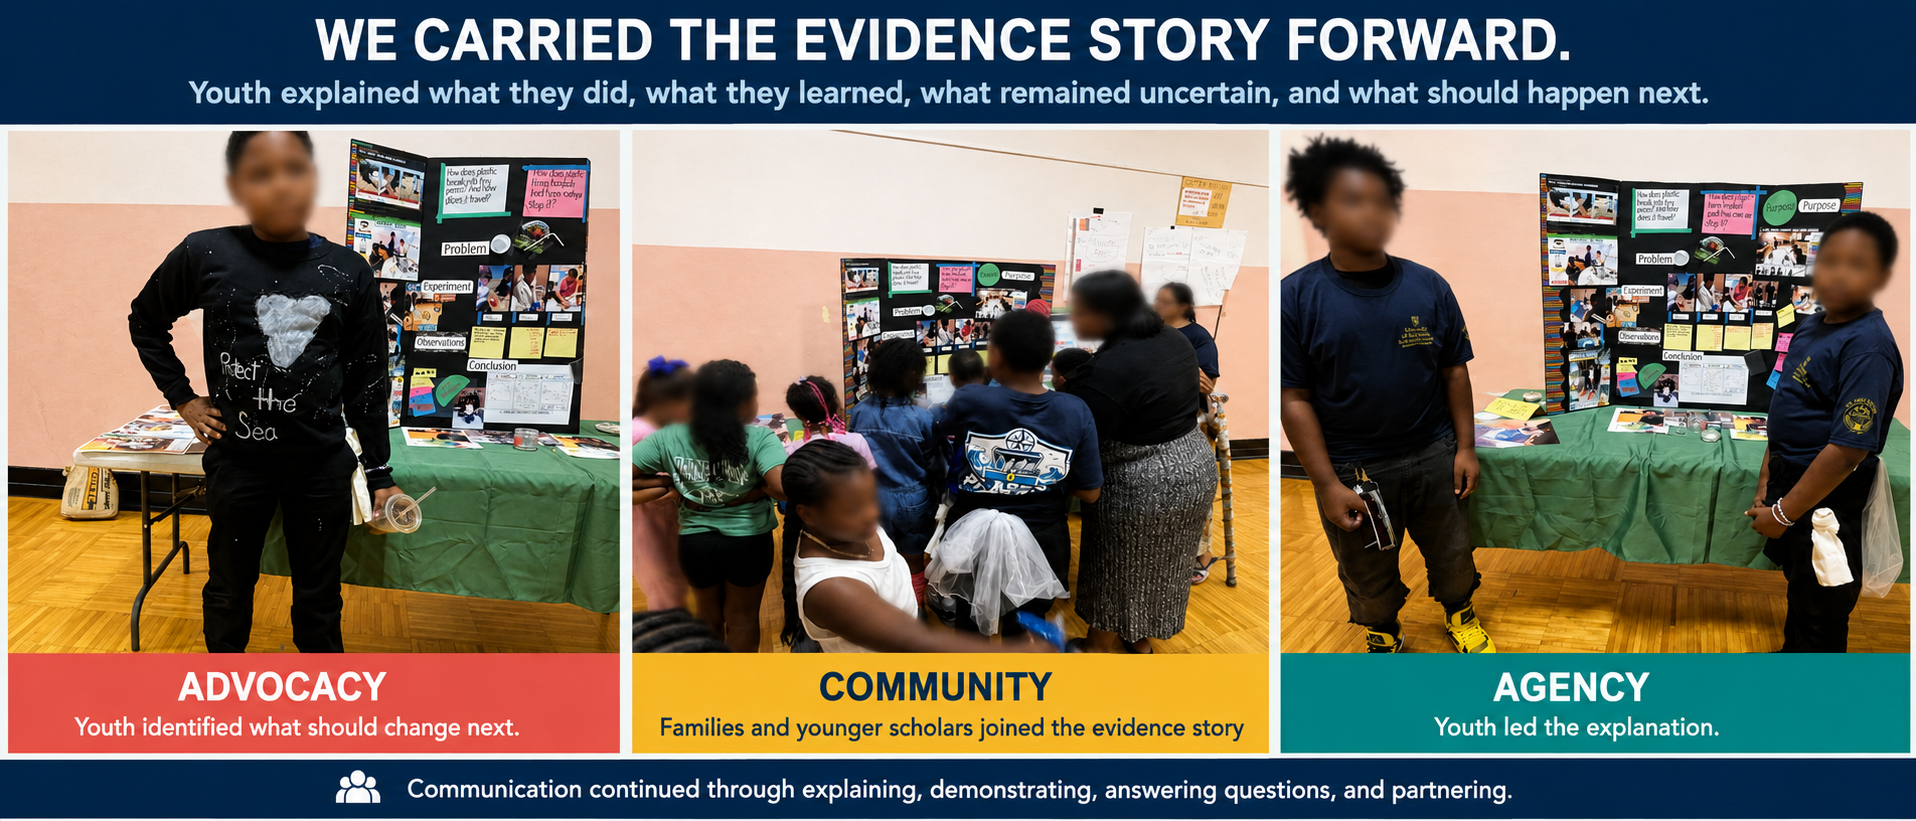
\includegraphics[
  width=0.8\textwidth,
  keepaspectratio
]{assets/artifact-previews/youth_carry_the_evidence_forward.png}

\parbox{1.0\textwidth}{\centering\textbf{\color{DeepNavy}Communication Continuity Beyond the Device.}
Youth carried the week's evidence into a new audience of families, visitors, and younger scholars. They explained, demonstrated, pointed, answered questions, partnered with others, and used the shared evidence display to reconstruct what they had done, what remained uncertain, and what they believed should happen next. Communication continued because the message could travel through different people and modes \citep{campEvidence2026}.}
\end{center}

\reflectionbox{\textbf{Practice artifact --- vocabulary from youth feedback:} Camp feedback showed why a backup system must include more than academic vocabulary. Youth identified smell and texture as barriers in the fish activity and proposed changes for future participation. A mask was one suggestion, but equipment does not equal consent. The context strip therefore includes \textit{smell, texture, observe only, no fish, different material,} and \textit{ready later} alongside science words. Those messages became design evidence: youth could communicate what should continue, what should change, and what future participants might need. A backup therefore preserves not only participation in the present activity, but the learner's ability to influence what happens next \citep{campEvidence2026}.}

\adaptationbox{A dense grid may be inaccessible because of vision, motor, literacy, language, sensory, or attention needs. Reduce field size, increase spacing or contrast, use photographs or objects, add partner-assisted scanning, or create layered displays while preserving robust message functions. Do not change symbol locations casually. Trial revisions with the communicator, and treat rejection of the board as information about the system rather than noncompliance. Continuity succeeds when the learner's meaning remains available even when the route, partner, activity, or audience changes.}

\sourcebox{ASHA AAC overview \citep{ashaAAC}; multimodal AAC design \citep{mirenda2015aids}; implementation context \citep{norrie2021context}; de-identified camp feedback/evidence.}